\documentclass[12pt,answers]{exam}

\usepackage[left=0.9in,right=0.9in,top=0.8in,bottom=1.05in]{geometry}
\newcommand{\ligne}[1]{\rule[0.5ex]{\textwidth}{#1}\\}

\usepackage[]{graphicx}
\usepackage{wrapfig}
\usepackage{physics}
\usepackage{float}

\begin{document}

\begin{center}
\textbf{Numerical PDEs Homework \#0}\\
\end{center}

\noindent \textbf{For all problems asking for a graph:} you do not need to write up the method you programmed. Including plots of your solution and convergence is sufficient for full credit. The ideal homework will have one, information-dense and properly labeled figure with a caption and a \textit{brief} discussion. \textbf{You must type up your HW.} I don't care if it's word or Tex as long as it's well organized, easy to follow, and submitted as a pdf. 

\vspace{0.3cm}

\noindent \textbf{Problem 1: Finite differences}
Write a matlab code that uses finite differences to compute the first derivative of
$$f(x) = \exp(\sin(x))$$
on the interval $0 \leq x \leq 2\pi$. Use second-order centered differences on internal grid points and first-order one-sided differences at endpoints. 
\begin{enumerate}
    \item Show a graph of the exact analytic solution $f'(x)$ and your numerical solution $f_n'(x)$. 
    \begin{solution}
    \begin{figure}[H]
    \centering
    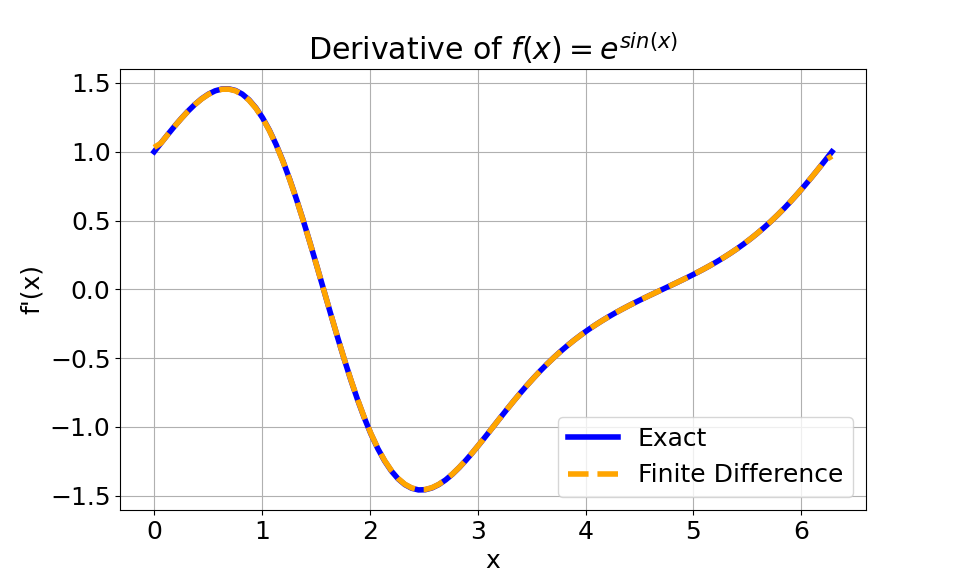
\includegraphics[width=1\textwidth]{fig/Problem1Part1.png}
    \caption{Comparison of the exact derivative of $f(x) = e^{\sin{(x)}}$ with the numerical finite-difference approximation, using second-order centered differences at interior points and first-order one-sided differences at the boundary points ($x =0$ and $x = 2 \pi$).}
    \label{fig:derivative}
\end{figure}
        Figure~\ref{fig:derivative} shows that the finite-difference approximation is visually indistinguishable from the exact derivative across the internal grid points. The end points slightly differ from the exact derivative. This is not surprising given that the endpoints use only first-order one-sided difference ($O(h)$ error), while the interior points use second-order centered difference ($O(h^2)$ error).
    \end{solution}
    \item Show a relative error convergence plot by plotting the relative error on the y-axis and the grid size $N$ on the x-axis. Measure relative error as 
    $$Err = \frac{\Vert f'(x) - f'_n(x) \Vert_p}{\Vert f'(x) \Vert_p}.$$
    \noindent Plot the error using both the $p=\infty,2$ norms in a log-log scale. The relative errors should be lines with slopes 1 and 3/2 respectively, i.e. it scales with $\displaystyle \frac{1}{N}, \frac{1}{N^{3/2}}$. Extra Credit: The $3/2$ slope is strange, why is that happening?
    \begin{solution}
        \begin{figure}[H]
            \centering
            
\includegraphics[width=1\linewidth]{fig/Problem1Part2.png}
            \caption{Convergence of Finite Difference First Derivative.}
            \label{fig:firstconvergence}
        \end{figure}
        Figure~\ref{fig:firstconvergence} shows that both the $L_{\infty}$ and $L_2$ relative errors decrease as N increases, confirming convergence of the finite-difference scheme. The $L_{\infty}$ error decreases with a slope of approximately $-0.97$, matching the expected first-order rate of $O(N^{-1})$, while the $L_2$ error decreases faster, with a slope of approximately $-1.55$, close to the expected $O(N^{-\frac{3}{2}})$ rate.
        
        \textbf{Extra Credit:}

        The $L_\infty$ error is set by the worst point, which is one of the two endpoints where the one-sided difference has $O(h)$ error, so $L_\infty \sim N^{-1}$. For $L_2$, summing squared errors gives $2\cdot O(h^2)$ from the two endpoints and $N\cdot O(h^4) = O(h^3)$ from the interior, so the endpoints dominate and $\Vert f' - f'_n \Vert_2 = O(h)$. The discrete 2-norm is an unweighted sum over $N$ points, so $\Vert f' \Vert_2 \sim \sqrt{N}$ grows with the grid, while the error is concentrated in only two points whose count does not grow. Dividing gives
        $$Err_2 \sim \frac{O(h)}{\sqrt{N}} = O(N^{-1}) \cdot O(N^{-1/2}) = O(N^{-3/2}).$$
        If the norm were scaled by $\sqrt{h}$ (a proper approximation to the continuous $L_2$ norm), the numerator would be $\sqrt{h}\cdot O(h) = O(h^{3/2})$ and the denominator would be $O(1)$, giving the same rate, the $3/2$ reflects $O(h)$ errors living on a set of measure $O(h)$.
    \end{solution}
\end{enumerate}

\vspace{0.5cm}

\noindent \textbf{Problem 2: Second-order derivatives}
Repeat problem 1 but compute the second derivative $f''(x)$. Assume periodicity and wrap around the grid instead of using one-sided finite differences.
\begin{solution}
    \begin{figure}[H]
        \centering
        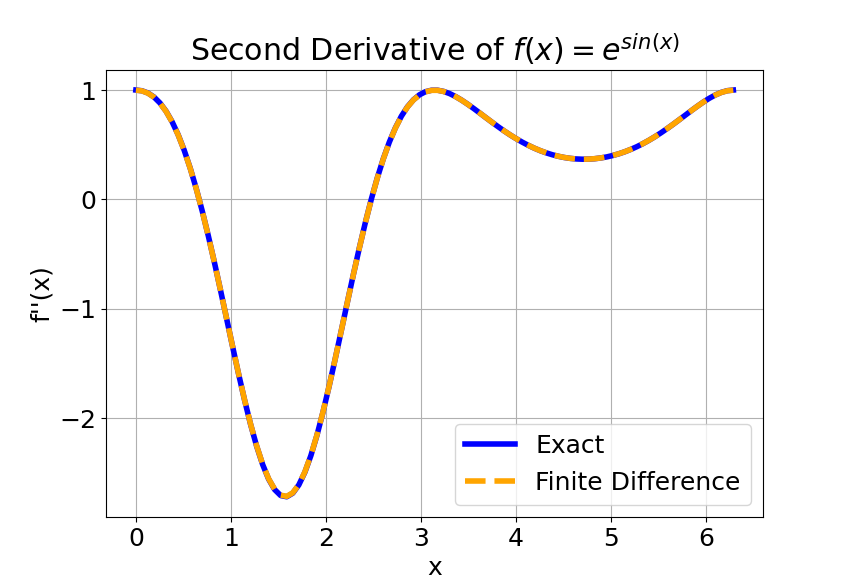
\includegraphics[width=1\linewidth]{fig/Problem2Part1.png}
        \caption{Comparison of the exact second derivative of $f(x) = e^{\sin (x)}$ with the numerical finite-difference approximation, using second-order centered differences at interior points and periodicity at the boundary points ($x =0$ and $x = 2 \pi$).}
        \label{fig:seconddev}
    \end{figure}
    Figure~\ref{fig:seconddev} shows that the numerical second derivative is visually indistinguishable from the exact second derivative function everywhere, including at the endpoints. Because the wrap-around treats $x = 0$ and $x = 2\pi$ as neighbors on a periodic grid, every point uses the second-order centered stencil and there is no first-order boundary error.
    \begin{figure}[H]
        \centering
        
\includegraphics[width=1\linewidth]{fig/Problem2Partb.png}
        \caption{Relative error of the periodic finite-difference second derivative versus $N$ (log-log), with reference slope $N^{-2}$.}
        \label{fig:secondconvergence}
    \end{figure}
    Figure~\ref{fig:secondconvergence} shows that the $L_{\infty}$ and $L_2$ relative errors both decrease with slopes of approximately $-2.01$ and $-2.04$, which match the expected $O(N^{-2})$ rate. Unlike, Problem 1, the two norms converge at the same rate, because periodicity removes the lower-order boundary error that caused the $3/2$ slope.
\end{solution}

\vspace{0.5cm}

\noindent \textbf{Problem 3: ODE}
Consider the ODE
$$\dv[2]{u}{x} + \sin(x) \dv{u}{x} + u(x) = f(x)$$
defined on $0 \leq x \leq 5$. Solve the ODE using second-order finite difference methods with the Dirichlet conditions. Use $u(x) = \sin(x)$ to test your solution by finding boundary conditions and the necessary forcing function $f(x)$. Show an error plot that proves your method converges with second order. 

\begin{solution}
    Substituting $u(x) = \sin (x)$ into the ODE gives $u'' = - \sin (x)$ and $\sin(x)u' = \sin(x) \cos(x)$, so
    \[f(x) = -\sin(x) + \sin(x) \cos(x) + \sin(x) =  \sin(x) \cos(x)\]
    with Dirichlet conditions $u(0) = 0$ and $u(5) = \sin (5)$.
    \begin{figure}[H]
        \centering
        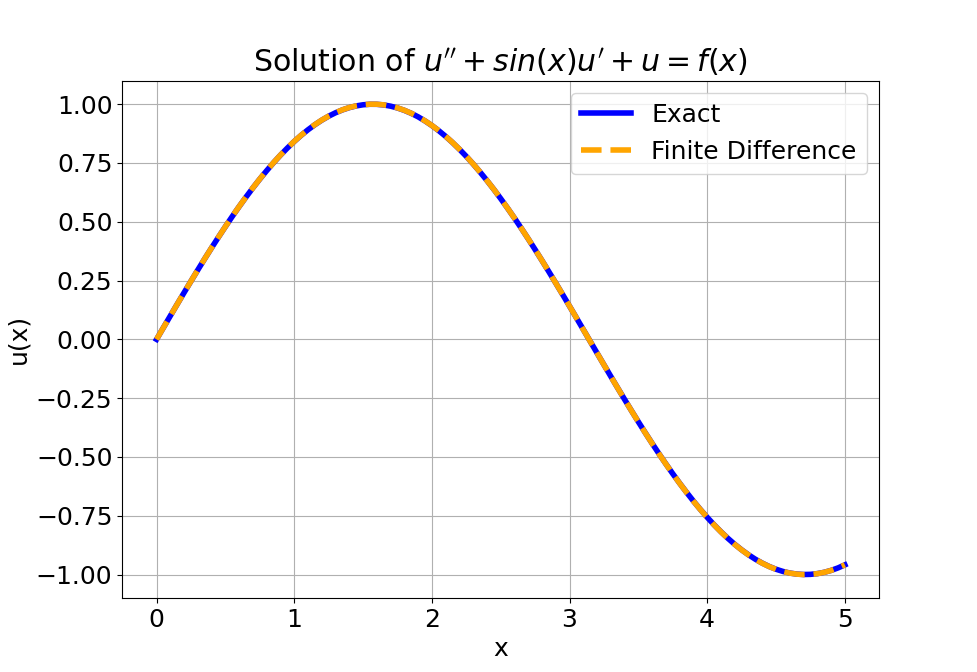
\includegraphics[width=1\linewidth]{fig/Problem3Part1.png}
        \caption{Solution to $u'' + \sin (x) u' + u = f(x)$, where $u = \sin (x)$ and $0 \leq x \leq 5$.}
        \label{fig:odesolved}
    \end{figure}
    Figure~\ref{fig:odesolved} shows that the numerical solution is visually indistinguishable from the exact solution across the whole domain.
    \begin{figure}[H]
        \centering
        
\includegraphics[width=1\linewidth]{fig/Problem3Part2.png}
        \caption{Relative error of the finite-difference ODE solution versus $N$ (log-log), with reference slope $N^{-2}$.}
        \label{fig:thirdconvergence}
    \end{figure}
    Figure~\ref{fig:thirdconvergence} shows that the $L_{\infty}$ and $L_2$ relative errors decrease with slopes of approximately $-2.03$ and $-2.01$, confirming that the method converes with second order.
\end{solution}

\vspace{0.5cm}
\noindent \textbf{Problem 4: Poisson Equation}
Use finite difference methods to solve the Poisson equation $\nabla^2 u = f(x,y)$ in the domain $x \in [0, 5], y \in [0, 5]$. Use the test solution $u(x,y) = \sin(x)\cos(y)$. 

\begin{enumerate}
    \item Apply Dirichlet conditions on all boundaries so that $u(x,y)$ satisfies the PDE and the boundary conditions, and show a plot of your solution and a second order convergence plot (similar to the first three problems). 
    \begin{solution}
    For the test solution, $\nabla^2 u = - \sin (x) \cos (y) - \sin(x) \cos(y)$, so $f(x, y) = - 2\sin(x) \cos (y)$. 
        \begin{figure}[H]
            \centering
            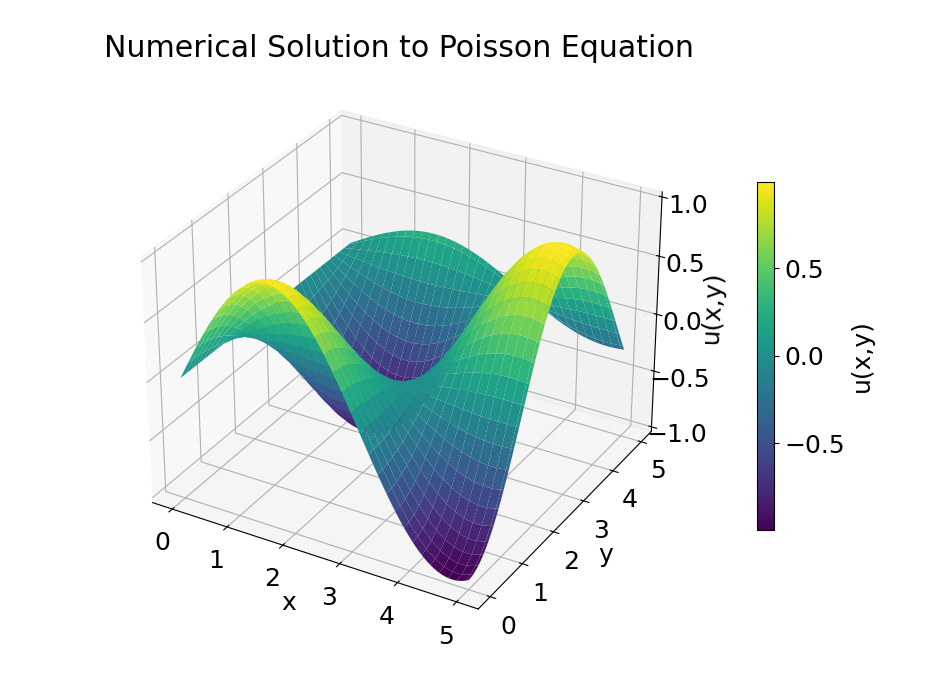
\includegraphics[width=1\linewidth]{fig/Problem4Part1.png}
            \caption{Numerical Solution to Poisson Equation for $u(x, y) = \sin (x) \cos (y)$}
            \label{fig:problem4part1}
        \end{figure}
        Figure~\ref{fig:problem4part1} shows the numerical solution to the 2D Poisson equation with Dirichlet boundary conditions, computed on the domain $[0, 5] \times [0, 5]$ with $N = 100$. The solution exhibits the same oscillatory pattern of $u(x,y) = \sin (x) \cos(y)$, with two peaks yellow, $u \approx 1$ and dark purple at $u \approx -1$. The solution stays bounded within $[-1, 1]$ as expected from the exact solution's range.
        \begin{figure}[H]
            \centering
            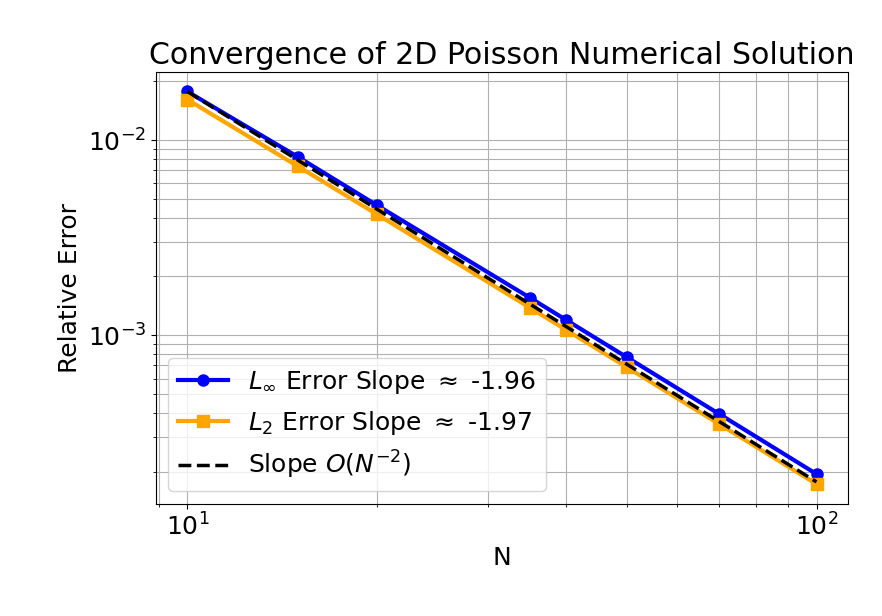
\includegraphics[width=1\linewidth]{fig/Problem4Part2.png}
            \caption{Relative error of the 2D Poisson solution with Dirichley conditions versus $N$ (with $N_x = N_y = N$), log-log, with reference slope $N^{-2}$.}
            \label{fig:problem4part2}
        \end{figure}
        Figure~\ref{fig:problem4part2} shows the relative error as a function of $N$ on a log-log scale. The $L_{\infty}$ and $L_2$ errors decreases with slopes of approximately $-2.00$ and $-1.97$, validating second-order convergence.
    \end{solution}
    \item Modify your code to apply Neumann conditions on all boundaries. \textbf{This won't work.} Why not? -- both in terms of the linear algebra and in terms of the actual PDE we want to solve. Suggest a solution to the issue.
    \begin{solution}
For the Neumann condition, we use the derivatives of the test solution as the boundary data. The partial derivatives of the test solution are 
\begin{align*}
    \frac{\partial u}{\partial x} = \cos (x) \cos(y) \qquad  \frac{\partial u}{\partial y} = -\sin (x) \sin (y)
\end{align*}
If $u$ solves $\nabla^2 u = f$ with $\frac{\partial u}{\partial n} = g$ on the boundary, then so does $u + C$ for any constant $C$, since neither the Laplacian nor the normal derivative sees a constant. The solution is therefore not unique. There is also a condition for a solution to exist at all. Integrating the PDE and applying the divergence theorem gives 
\[\int_{V} f \, dV = \int_{V} \Delta u \, dV = \int_{S} \frac{\partial u}{\partial n} \, dA\]
so the forcing function and the boundary data cannot be chosen independently. Physically, for steady heat conduction with prescribed fluxes, the total source inside must balance the total flux through the boundary. With Neumann conditions, every row of the Laplacian sums to zero, so $L\mathbf{1} = \mathbf{0}$, which means the constant vector is in the null space and $L$ is singular and can't be inverted.

To fix this, we can pick one grid point and set $u$ there to a known value. We use the corner $(0,0)$ and replace its equation with $u_{0,0} = u(0,0) = 0$, just like a Dirichlet condition at a single point. 

    \end{solution}
\end{enumerate}

\end{document}